
\mychapter{Medium}{Medium}
We chose to make our medium, both rod and surrounding liquid, a changeable parameter to see
the influence of the density difference and the liquid's viscosity on the process. First of all, we see
that depending on the sign of the density difference, we get either sedimentation or a collection and ordering of the particles at that top of the liquid. We primarily used iron and lithium as rod
material as they demonstrate this change of sign when paired up with water as the surrounding
material. Interestingly, while iron has eight times the density of water and lithium is much closer at half of the water’s density, this does not seem to make a huge difference in the timescales of the
process. Though iron seems to order itself slower, so the tendency is there.\\
\begin{figure}[h]
  \begin{minipage}[t]{0.45\textwidth}
    \fbox{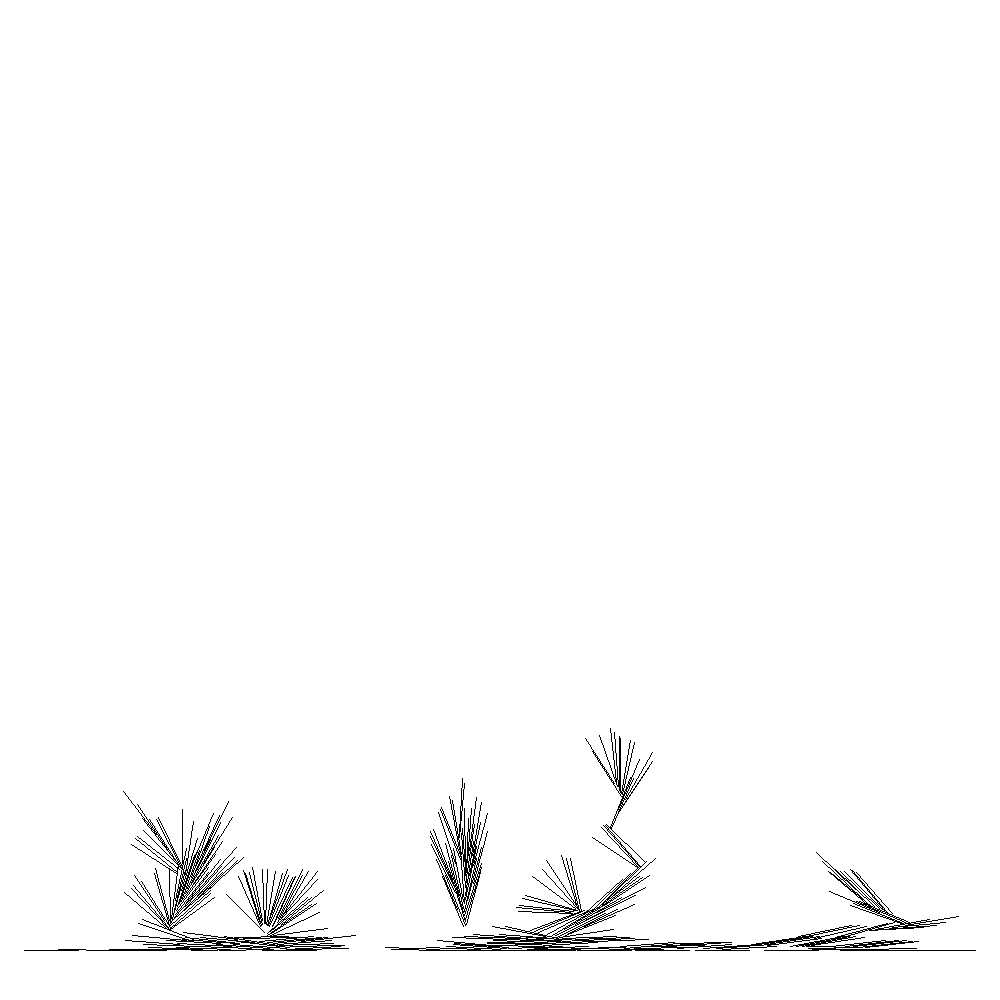
\includegraphics[width=\textwidth]{data/med_comp1_L.png}}
  \end{minipage}
  \hfill
  \begin{minipage}[t]{0.45\textwidth}
    \fbox{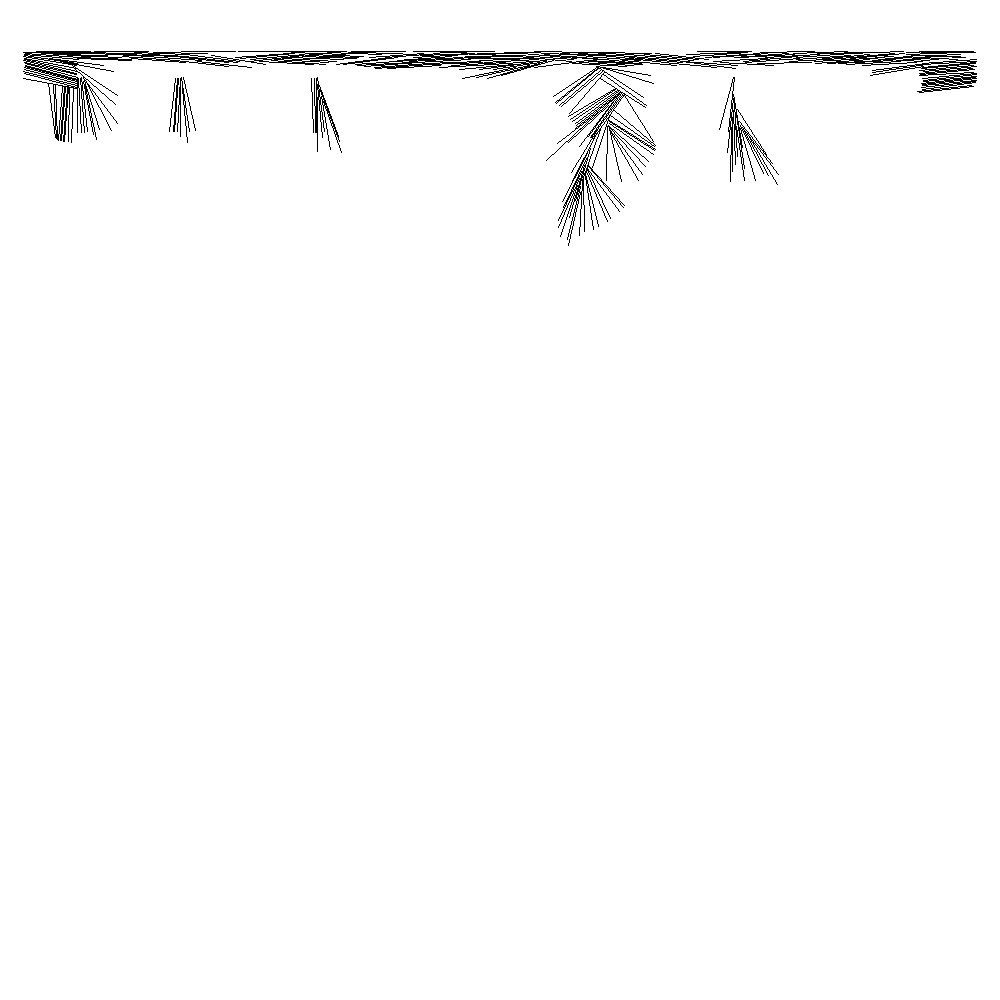
\includegraphics[width=\textwidth]{data/med_comp1_R.png}}
  \end{minipage}
  \caption{Comparison of iron (left) and lithium (right) rods in water, picture shows end state after 5e8 MC iteration steps. We can see that the lithium gathers at the top, while iron due to it's larger then water density gathers at the bottom.}
  \label{fig:med_comp1}
\end{figure}
\begin{figure}[h]
\begin{minipage}[tc]{0.50\textwidth}
    \hspace{-0.2\textwidth}
    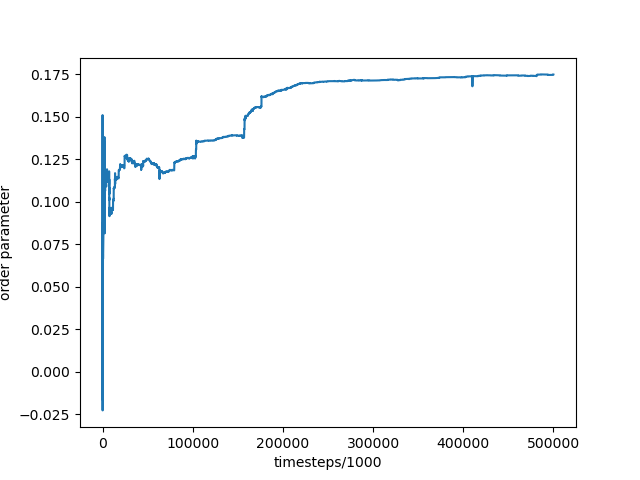
\includegraphics[width=1.3\textwidth]{data/med_comp2_L.png}
  \end{minipage}
  \hfill
  \begin{minipage}[tc]{0.50\textwidth}
    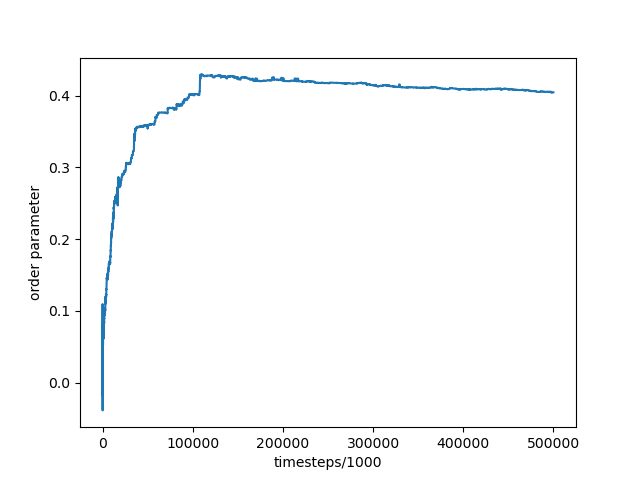
\includegraphics[width=1.3\textwidth]{data/med_comp2_R.png}
  \end{minipage}
    \caption{Comparison of iron (left) and lithium (right) rods in water and their respective order parameters. A slightly faster ordering can be seen on the lithium graph, though that could just be incidental.}
  \label{fig:med_comp2}
\end{figure}
As an alternative liquid than water, we choose honey. Our main result there was that the entire process slows down as the higher viscosity dampens movement.
\begin{figure}[h]
  \begin{minipage}[t]{0.45\textwidth}
    \fbox{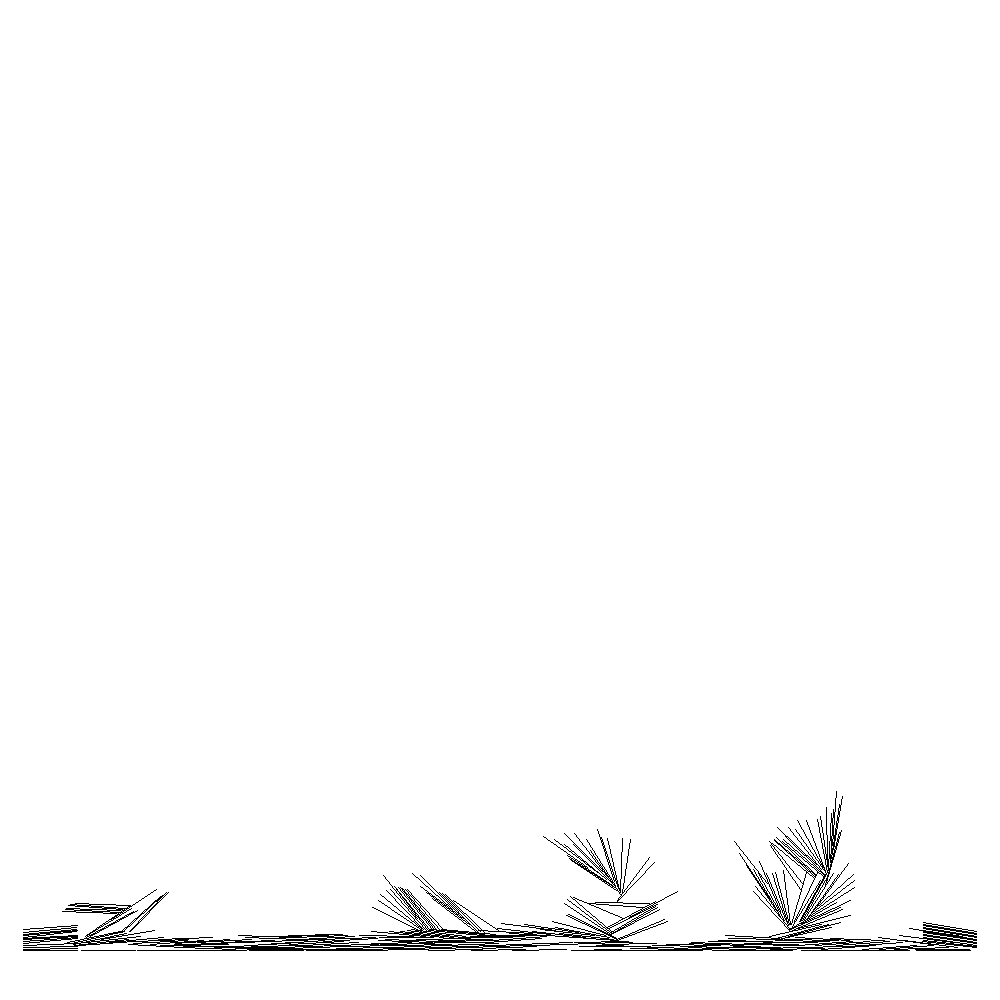
\includegraphics[width=\textwidth]{data/med_comp3_L.png}}
  \end{minipage}
  \hfill
  \begin{minipage}[t]{0.45\textwidth}
    \fbox{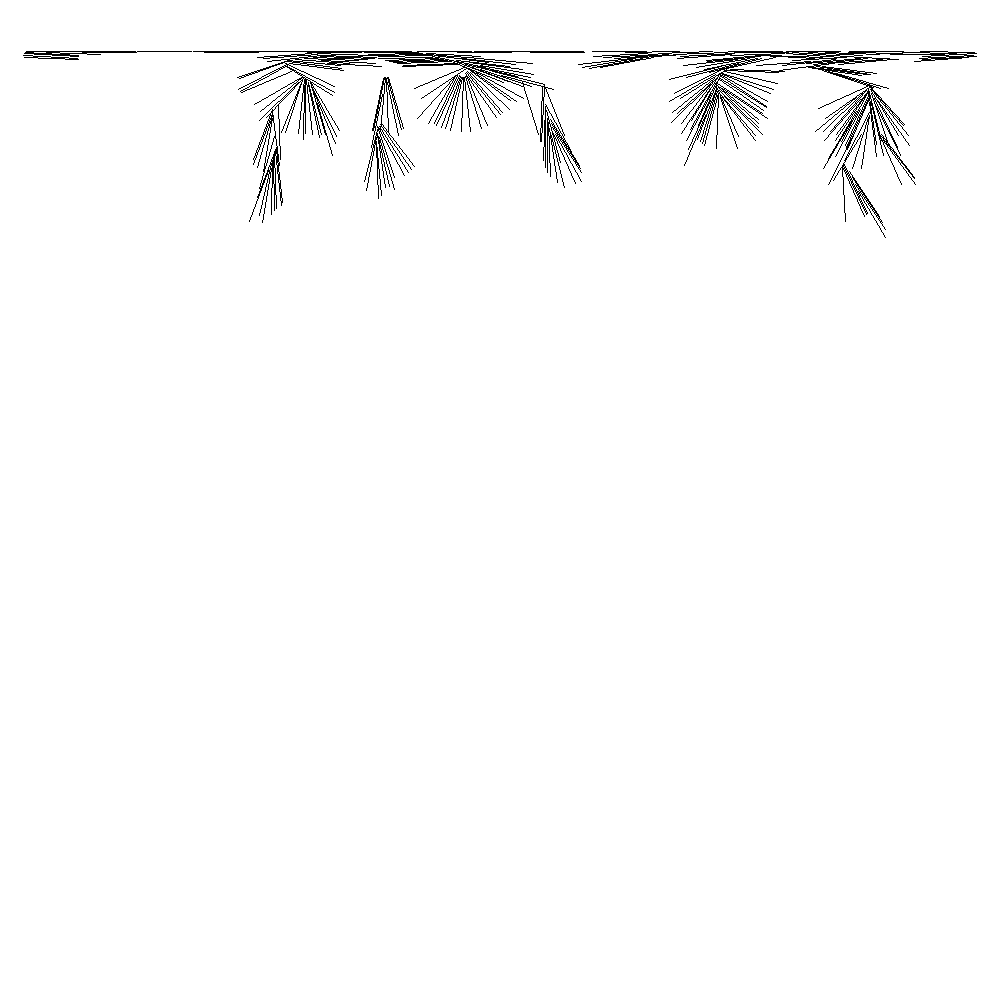
\includegraphics[width=\textwidth]{data/med_comp3_R.png}}
  \end{minipage}
  \caption{Comparison of iron (left) and lithium (right) rods in honey, picture shows end state after 5e8 MC iteration steps. Similar to \ref{fig:med_comp1} though the ordering seems to not have progressed thus far due to the biger viscosity of the honey.}
  \label{fig:med_comp3}
\end{figure}
\begin{figure}[h]
  \begin{minipage}[tc]{0.50\textwidth}
    \hspace{-0.2\textwidth}
    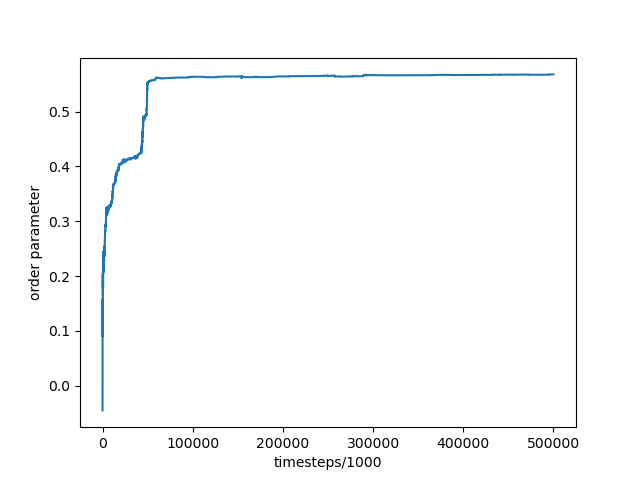
\includegraphics[width=1.3\textwidth]{data/med_comp4_L.png}
  \end{minipage}
  \hfill
  \begin{minipage}[tc]{0.50\textwidth}
    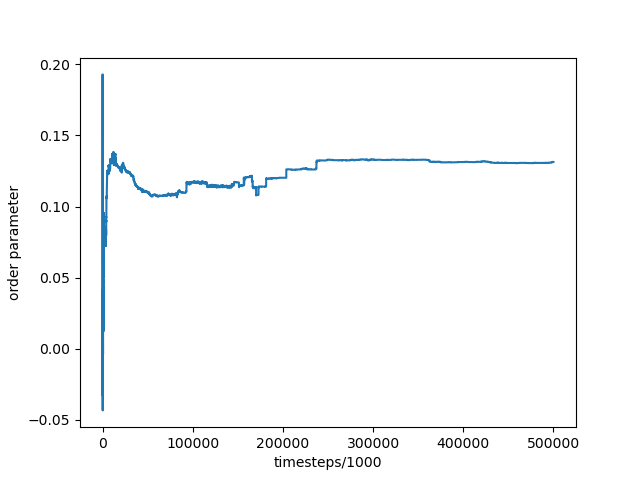
\includegraphics[width=1.3\textwidth]{data/med_comp4_R.png}
  \end{minipage}
  \caption{Comparison of iron (left) and lithium (right) rods in honey and their respective order parameters. This time, the iron rods seem to order slightly faster which further suggests that these trends are mere incidental.}
  \label{fig:med_comp2}
\end{figure}



\clearpage
